\chapter{State of the Art}
\label{theory}
\thispagestyle{plain}

In this section, we review the state of the art of problem at hand. We start by describing why timetabling is a rather complex problem, some possible approaches on trying to solve the problem and some of the solutions already taken, specifically for the ITC 2007 benchmarks.
\\
%%%%%%%%%%%%%%%%%%%%
\section{Timetabling Problem}
%%%%%%%%%%%%%%%%%%%%
When solving timetabling problems, it is possible to generate one of multiple types of solutions which are named \textit{feasible solutions}, \textit{non feasible solutions}, \textit{optimal solutions} or \textit{sub-optimal solutions}. A feasible solution is a solution that solves all the mandatory problem constraints, in contrary to non feasible solutions. An optimal solution is the best feasible solution possible considering the problem and its optimal solution value. It's possible for a problem to have multiple optimal solutions. For last, non-optimal solutions are feasible solutions that can't reach the optimal solution value and so are not as good compared to an optimal solutions.\\

Timetabling automation is a subject that has been a target of research for about 50 years. The timetabling problem may be formulated as a search or optimization problem~\cite{Schaerf1999}. As a search problem, the goal consist on finding a solution (feasible solution) that satisfies all the hard constraints, while ignoring the soft constraints. On the contrary, posing the timetabling problem as an optimization problem, one seeks to minimize (considering a minimization problem) the violations of soft constraints while satisfying the hard constraints. Typically, the optimization is done after using a search procedure for finding an initial feasible solution.\\

The basic examination timetabling problem, where only the clash (conflict) hard constraint is observed, reduces to the graph coloring problem~\cite{Jensen2001}. This is a well studied hard problem. Deciding whether a solution exists in the Graph Coloring problem is a NP-complete problem~\cite{Arora2009}. Considering the graph coloring as an optimization problem, it is proven that the task of finding the optimal solution is a NP-Hard problem~\cite{Arora2009}. Graph Coloring problems are explained further in~\ref{subsection:ExistingAppr}
\\
%%%%%%%%%%%%%%%%%%%%
\section{Existing approaches}
\label{subsection:ExistingAppr}
%%%%%%%%%%%%%%%%%%%%
\begin{figure}[h!]
 \centering
   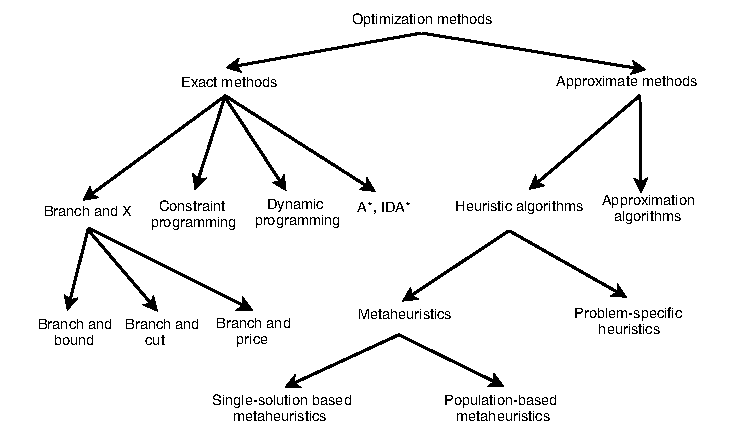
\includegraphics{./images/typesOfAlgorithms}
   \caption{Types of algorithms adapted from \cite{Talbi2009}.}
   \label{fig:TypesAlgorithms}
\end{figure}

The Figure~\ref{fig:TypesAlgorithms} represents the organization of Optimization methods. These methods are divided into \textit{Exact methods} and \textit{Approximate methods}.\\

Timetabling solution approaches are usually divided in the following categories~\cite{Qu2009}: \textit{exact algorithms} (Branch-and-Bound, Dynamic Programming), \textit{graph based sequential techniques}, \textit{local search based techniques} (Tabu Search, Simulated Annealing), \textit{population based algorithms} (Evolutionary Algorithms, Memetic algorithms, Ant algorithms, Artificial immune algorithms), \textit{Multi-criteria techniques}, \textit{Hyper-heuristics}, \textit{Decomposition/clustering techniques} and \textit{Hybrid algorithms}, which combine features of several algorithms, comprise the state-of-the-art. Due to its complexity, approaching the examination timetabling problem using exact method approaches can only be done for small size instances. Real problem instances found in practice are usually of large size, making the use of exact methods impracticable. Heuristic solution algorithms have been usually employed to solve this problem.\\

Real problem instances are usually solved by applying algorithms which use both \textit{heuristics} and \textit{meta-heuristics}. Heuristic algorithms are problem-dependent, meaning that these are adapted to a specific problem in which take advantage of its details. Heuristics are used to generate a feasible solution, focusing on solving all hard constraints only. Meta-heuristics on the other hand are problem-independent. These are used to, given the feasible solution obtained using heuristic algorithms, generate a better solution focusing on solving as many soft constraints as possible.\\
\\
Most of the Meta-heuristic algorithms used belong to one of the three categories: One-Stage algorithms, Two-Stage algorithms and algorithms that allow relaxations~\cite{Lewis2007}. 
\begin{itemize}
  \item The One-Stage algorithm is used to get an initial optimal solution, which the goal is to satisfy both hard and soft constraints at the same time. Approaches using this stage are not very common because it's hard to get proper solutions in a reasonable amount of time trying to satisfy both types of constraints at the same time;
  \item The Two-Stage algorithms are the most used types of approaches This category is divided in two phases. The first phase consists in all soft constraints being "discarded" and focus only on solving hard constraints to obtain a feasible solution. The next phase is an attempt to find the best solution, trying to solve the highest number of soft constraints possible given the solution of the first phase.
\end{itemize}

\subsection{Exact methods}
\label{subsection:exactmethods}
Approximation algorithms like Heuristics and meta-heuristics proceed to enumerate partially the search space and, for that reason, they can't guarantee finding the optimal solution. On the other side, exact approaches perform a complete enumeration of the search space and thus guarantee that the encountered solution is optimal. A negative aspect is the time taken to find the solution. If the decision problem is very difficult (e.g. NP-Complete), in practical scenarios, if the size of the instances is large, this approach may not be applied due to the long execution time.\\

\paragraph{Constraint Programming Based Technique}
The Constraint Programming Based Technique (CPBT) allows direct programming with constraints which gives ease and flexibility in solving problems like timetabling. Two important features about this technique are backtracking and logical variables that facilitate searching for an optimal solution at the expense of time. Constraint programming is different from other types of programming, as in these types it is specified the steps that need to be executed, but in constraint programming it is specified the properties (hard constraints) of the solution or properties that should not be in the solution~\cite{Qu2009}.\\

\paragraph{Integer Programming}
The Integer Programming (IP) is a mathematical programming technique in which the optimization problem to be solved must be formulated as an Integer Linear Problem, that is, the objective function and the constraints must be linear, and all problem variables are integer valued. If there are some variables that are continuous and other are integer, then the problem is called Mixed-Integer Linear Programming (MILP). Schaerf~\cite{Schaerf1999} surveys some approaches using the MILP technique to school, course, and examination timetabling.

\subsection{Graph Coloring Based Techniques}
\label{subsection:graphcoloring}
Timetabling problems can be reduced to a graph coloring problem. The usual approaches use graph coloring heuristics in the first phase of the two-stage algorithms. Graph Coloring itself is not an heuristic or meta-heuristic but a method that designates a problem and its variants.\\

\paragraph{Graph Coloring Problem}
The Graph Coloring (GC) problems consists about assigning colors to an element type of the graph which corresponds to a constraint. The simplest sub-type is the \textit{vertex coloring}, which the main goal is to, given a number of vertices and edges, color the vertices so that no adjacent vertices have the same color. In this algorithm, it's best to find a solution with the lowest number of colors as possible. In examination timetable problem, a basic approach could be to represent the exams as vertices and the hard constraints as edges (considering this is search algorithm, it is good to use optimization algorithms to deal with soft constraints) so that exams with the same color, can be assign to the same timeslot. After coloring, it proceeds to assign the exams into timeslots considering the colors of the solution~\cite{Qu2009}.\\

Graph Coloring heuristics like \textit{Saturation Degree Ordering} are very commonly used to get the initial solutions. Others like \textit{First Fit}, \textit{Degree Based Ordering}, \textit{Largest Degree Ordering}, \textit{Incident Degree Ordering} are also heuristic techniques for coloring graphs~\cite{Lee1996}.\\

%\paragraph{Saturation Degree Ordering}
%The Saturation Degree Ordering heuristic colors the vertices with more constraints first. The coloring method is as follows: while choosing a vertice to color, the ones with higher saturation degree will be colored first. The saturation degree of one vertice is the number of differently colored vertices adjacent to this vertice or, in another words, the number of different colors of all adjacent vertices. In the case of a tie, the highest saturation vertice with higher number of adjacent vertices is chosen.

\subsection{Meta-heuristics}
Meta-heuristics, as mentioned above, usually provide solutions for optimization problems. In timetabling problems, meta-heuristic algorithms are used to optimize the feasible solutions provided by heuristics, like the GC. Meta-heuristics are divided in two main sub-types, which are \textit{Single-solution meta-heuristics} and \textit{Population-based meta-heuristics}~\cite{Talbi2009}.\\

\paragraph{Single-solution meta-heuristics}
Single-solution meta-heuristics' main goal is to modify and optimize one single solution, maintaining the search focused in local regions. This type of meta-heuristic is therefore exploitation oriented. Some examples of this type are \textit{SA}, \textit{Variable-Neighborhood Search}, \textit{Tabu Search}, \textit{Guided Local Search}~\cite{Talbi2009}. \\

\paragraph{Population-based meta-heuristics}
Population-based meta-heuristics' main goal is to modify and optimize multiple candidate solutions, maintaining the search focused in the whole space. This type of meta-heuristic is therefore exploration oriented. Some examples of this type are \textit{Particle Swarm}, \textit{Evolutionary Algorithms}, \textit{Genetic Algorithms}~\cite{Talbi2009}.\\

The common types of algorithms and how they are organized, are displayed in Figure~\ref{fig:TypesAlgorithms}


\subsection{ITC 2007 Examination timetabling problem: some approaches}
\label{subsection:ApprITC2007}

In this section the significant techniques applied to the ITC 2007 - Examination timetabling track are described. \\
This timetabling problem comprises 12 instances of different degree of complexity. Through the available website, competitors could submit their solutions for the given benchmark instances. Submitted solutions are evaluated in the following form. First, it is checked if the solution is feasible and a so-called distance to feasibility is computed. If it is feasible, the solution is further evaluated based on the fitness function, which measures the soft constraints total penalty. Then, competitors' solutions are ranked based on the distance to feasibility and solution's fitness value. The competitor with lower distance to feasibility value is the winner. In the case of a tie, the competitor's solution with the lowest fitness value wins. A solution is considered feasible if the value of distance to feasibility is zero. The set of hard constraints is the following:
\begin{itemize}
	\item no student must be elected to be present in more than one exam at the same time;
	\item the number of students in a class must not exceed the room's limit capacity;
	\item exam's length must not surpass the length of the assigned timeslot;
	\item exams ordering hard constraints must be followed - e.g., $Exam_1$ must be scheduled after $Exam_2$;
	\item room assignments hard constraints must be followed - e.g., 	$Exam_1$ must be scheduled in the $Room_1$.
\end{itemize}

It is also necessary to compute the fitness value of the solution and so consider the soft constraints that were not obeyed. The soft constraints are listed below:
\begin{itemize}
	\item two exams in a row: A student should not be assigned to be in two adjacent exams in the same day;
	\item two exams in a day: A student should not be assigned to be in two non adjacent exams in the same day;
	\item period spread: Reduce the number of times a student is assigned to be in two exams that are \textit{N} timeslots apart;
	\item mixed durations: Reduce the number of exams with different durations that occur in a room and period;
	\item larger exams constraints: Reduce the number of large exams that occur later in the timetable;
	\item room penalty: Avoid assigning exams to rooms with penalty;
	\item period penalty: Avoid assigning exams to periods with penalty.
\end{itemize}

To get a detailed explanation on how to compute the values of fitness and distance to feasibility based on the weight of each constraint, please check ITC 2007's website~\cite{McCollum2008}\\

The finalists are ranked based their rankings on the instances. For full details on the rankings system, please consult~\cite{BarryMcCollum2008}.\\

In this thesis, I'll be reviewing some of the winners approaches. The winners list of the ITC 2007 competition is as follows:
\begin{itemize}
	\item 1st Place: Tom\'{a}\v{s} M\"{u}ller
	\item 2nd Place: Christos Gogos
	\item 3rd Place:Mitsunori Atsuta, Koji Nonobe, and Toshihide Ibaraki
	\item 4th Place: Geoffrey De Smet
	\item 5th Place: Nelishia Pillay
\end{itemize}

\paragraph{Tom\'{a}\v{s} M\"{u}ller's approach:}

Tom\'{a}\v{s} M\"{u}ller's approach~\cite{Mueller2009} was actually used to solve all three problems established by the ITC 2007 competition. He was able to win two of them and be finalist on the third. For solving the problems, he opted for an hybrid approach, organized in a two-phase algorithm..\\
\\
In the first phase, Tom\'{a}\v{s} used Iterative Forward Search (IFS) algorithm~\cite{Mueller2005} to obtain feasible solutions and Conflict-based Statistics~\cite{Rudova2004} to prevent IFS from looping. The timetabling problems solved were specified as constraint satisfaction problems, where events (exams, courses) are represented by variables. The variables' values are the possible pairs (time slot, room) that don't cause violations in the hard constraints. For each iteration there's an attempt to sign a value to an unassigned variable. If it violates hard constraints, the conflicting variables are unassigned. The variable chosen in each iteration is randomized or parameterized to, for example, assign the most difficult assignable exam first. The Conflict-based Statistics was used to memorize some previously passed conflicts and avoid repeating those for each iteration.\\
\\
The second phase consists in using multiple optimization algorithms. These algorithms are applied using this order: HC~\cite{Russell2010}, Great Deluge (GD)~\cite{Dueck1993} and optionally SA~\cite{Kirkpatrick1983}.\\
\\
HC is used to optimize the first phase solution, resulting on a solution stuck at a local optimum. To leave local optimum area, GD is used in order to try and result in a better solution. For last, SA is used in a loop, keeping the temperature limit unchanged. After not getting a better solution for a limited time, the temperature is reheated (temperature limit gets higher) and HC phase is used again forming a loop in these 3 optimization algorithms.\\
\\
\paragraph{Christos Gogos' approach:}

Gogos was able to reach second place in Examination Timetabling track, right after Muller. Gogos' approach is very different compared to Muller's. His approach, like Muller's, was divided in two phases named \textit{Construction Phase} and \textit{Improvement Phase}, in which the first is used do construct a feasible solution and the second improves the solution found in the first phase, using local search algorithms.\\
\\
In the first phase, is starts using a Pre-processing stage. This stage deals with hidden dependencies, which means it adds dependencies to the problem that weren't there at the beginning but they exist and makes sense in the problem itself. For example, one hidden dependency may be one exam $E_1$ having an ordering constraint with exam $E_2$ stating that $E_2$ must be scheduled after exam $E_1$ and exam $E_3$ must be scheduled after exam $E_2$. So a dependency/constraint must be added so exam $E_3$ must be scheduled after exam $E_1$ as well. The key idea is that this pre-process method will be very helpful in the further stages when trying to find solutions.\\
\\
After the pre-processing stage, a construction stage takes place. This method is used to create a complete timetable. In this stage, multiple solutions are attempted considering the available time in which only the best solution is passed to the next phase. The solution is constructed by constantly setting an exam and a room to a period until a feasible solution is found.\\
\\
In the second phase, HC is used. This algorithm is used to generate neighbor solutions, accepting only better solutions compared to the current one, until reaching a local optimum. It is considered local optimum when HC cannot generate a better solution in a number of tries or time limit.\\
\\
The next stage consists in utilizing SA to get out of local maximum. Simulated Annealing stops when it cannot generate better solutions after the specified period of time.\\
\\
After Simulated Annealing, an IP formulation that uses Branch and Bound (BB) is used in a set of sub-problems. This stage is called "IP Sub-Problems Stage". This simply examines all periods trying to discover some possible improvements that can be done, for instance, swapping a room with high penalty with a room with no penalty or having lower penalty that is not currently being used.\\
\\
The last stage is the Shaking Stage. This method "shakes" the current best solution in order to get equally good solutions and pass it to SA stage. This method is not used if the problem we're solving only has one room or the cost of each room is zero. Two heuristics are used in this stage. The first creates neighbor solutions but a solution is only accepted if the new solution is equally good and the room arrangement is better (total cost of room assignment is lower) as compared to the current best solution. The second heuristic reschedule a set of exams presented on the previous solution. These are first removed from the timetable and then scheduled using the same techniques used in the construction stage. This heuristic will probably generate a worse solution but it is accepted and used next on the SA stage.\\
\\
Tabu Search (TS)~\cite{Talbi2009} is also used in this approach, even though it's not used as a standalone method. This one is used along with HC and SA algorithms to prevent them from looping and creating the same results. TS avoids the creation of equal neighbor solutions by not letting the same period be selected for swapping after this being selected once. This period can only be selected again after a certain number of swaps on other periods.\\
\\
